\chapter{知识图谱管理所使用的背景知识}
\section{图论}
过去几十年间,人们对现代社会发展中形成的``连通性''产生了日益浓厚的兴趣。这种兴趣的核心就是\emph{图}(graph)。图是事物之间相互关系的一种模式,人们在很多场合的讨论和报道中都会提到。实际应用中,已经出现了各式各样的图,如社交网络、知识图谱等等。这些图规模巨大,结构复杂,包含丰富的信息,为帮助人们更好地生产生活提供了丰富的信息源。


为此,本章将主要从图论的角度来作为知识图谱的基础知识。

\subsection{图的基本定义}
图论作为网络的基础最早是由瑞士著名数学家欧拉针对哥尼斯堡七桥问题所提出的。如今,图论已经成为了离散数学的一个重要分支,被广泛地在应用在各个领域。


\begin{example}
\textbf{哥尼斯堡七桥问题}
哥尼斯堡七桥问题是18世纪著名古典数学问题之一,欧拉通过求解这个问题奠定了图论。在哥尼斯堡的一个公园里,有七座桥将普雷格尔河中两个岛及岛与河岸连接起来(如图\ref{fig:graph:KnigsbergBridge}中左图所示)。问是否可能从这四块陆地中任一块出发,恰好通过每座桥一次,再回到起点?

\begin{figure}[htbp]
	\centering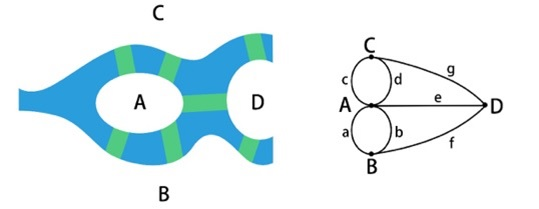
\includegraphics[width=3.5in]{./figures/part1/KnigsbergBridge.jpg}
	\caption{哥尼斯堡七桥问题示例图}\label{fig:graph:KnigsbergBridge}
\end{figure}

欧拉于1736年研究并解决了此问题,他把问题归结为如图\ref{fig:graph:KnigsbergBridge}中右图所示图上的``一笔画''问题。欧拉不仅解决了此问题,且给出了连通图可以一笔画的充要条件是:有奇数个相邻边的点不是没有就是两个。证明思路在于要想一笔画成,中间路过点必须均是偶数条相邻变,也就是有来路必有另一条去路,有奇数个相邻边的点要么没有要么在两端。
\end{example}



%\subsection{基本定义}\label{sec:graphdefinition}
这里所说的\emph{图},是以一种抽象的形式来表示若干对象结合以及这些对象之间的关系。


\begin{definition}
\label{def:graph}
\textbf{图}:图表示成一个二元组$G=(V,E)$,其中V 是点集合;E 表示边集合,其中每条边由V中两个点相连接所构成。构成一条边的两个点称之为这条边的端点。一条边的两个端点可以是V中的相同或者不同点,两个端点相同的边称之为\emph{环}。
\end{definition}

如果E中的边都是没有方向的,那么G被称为无向图;如果E中的边是有方向的,那么G被称为有向图。
给定V中的两个元素u和v,如果它们之间存在一条无向边,则记为$e=(u,v)\in E$;如果它们之间存在一条有向边,则记为$e=\langle u,v\rangle \in E$,其中u被称为起点,v被称为终点。
此外,G中的边$e$可以被赋上一个权重,记为$w(e)$。

\begin{definition}
\label{def:graph_degree}
\textbf{度数}:给定一个无向图$G=(V,E)$,对于任意的$v\in V$,称v作为G中边的端点的次数之和为v的\emph{度数},简称\emph{度},记作$deg_G(v)$,在不发生混淆的情况下,也可以简写为$deg(v)$。

给定一个有向图$G=(V,E)$,对于任意的$v\in V$,称v作为G中边的起点的次数之和为v的\emph{出度},记作$deg_G^+(v)$,简记作$deg^+(v)$;称v作为G中边的终点的次数之和为v的\emph{入度},记作$deg_G^-(v)$,简记作$deg^-(v)$。$deg^+(v)+deg^-(v)$被称为v的度数,记作$deg(v)$。
\end{definition}

\begin{example}
图\ref{fig:graph:ExampleGraph}给出了一个无向图和有向图的示例。其中,对于图\ref{fig:graph:ExampleGraphUndirected}中点3而言,它的度数是4;对于图\ref{fig:graph:ExampleGraphDirected}中点3而言,它的入度是3,出度是1,度数是4。

\begin{figure}[h]
   \centering
\subfigure[][{无向图}]{%
      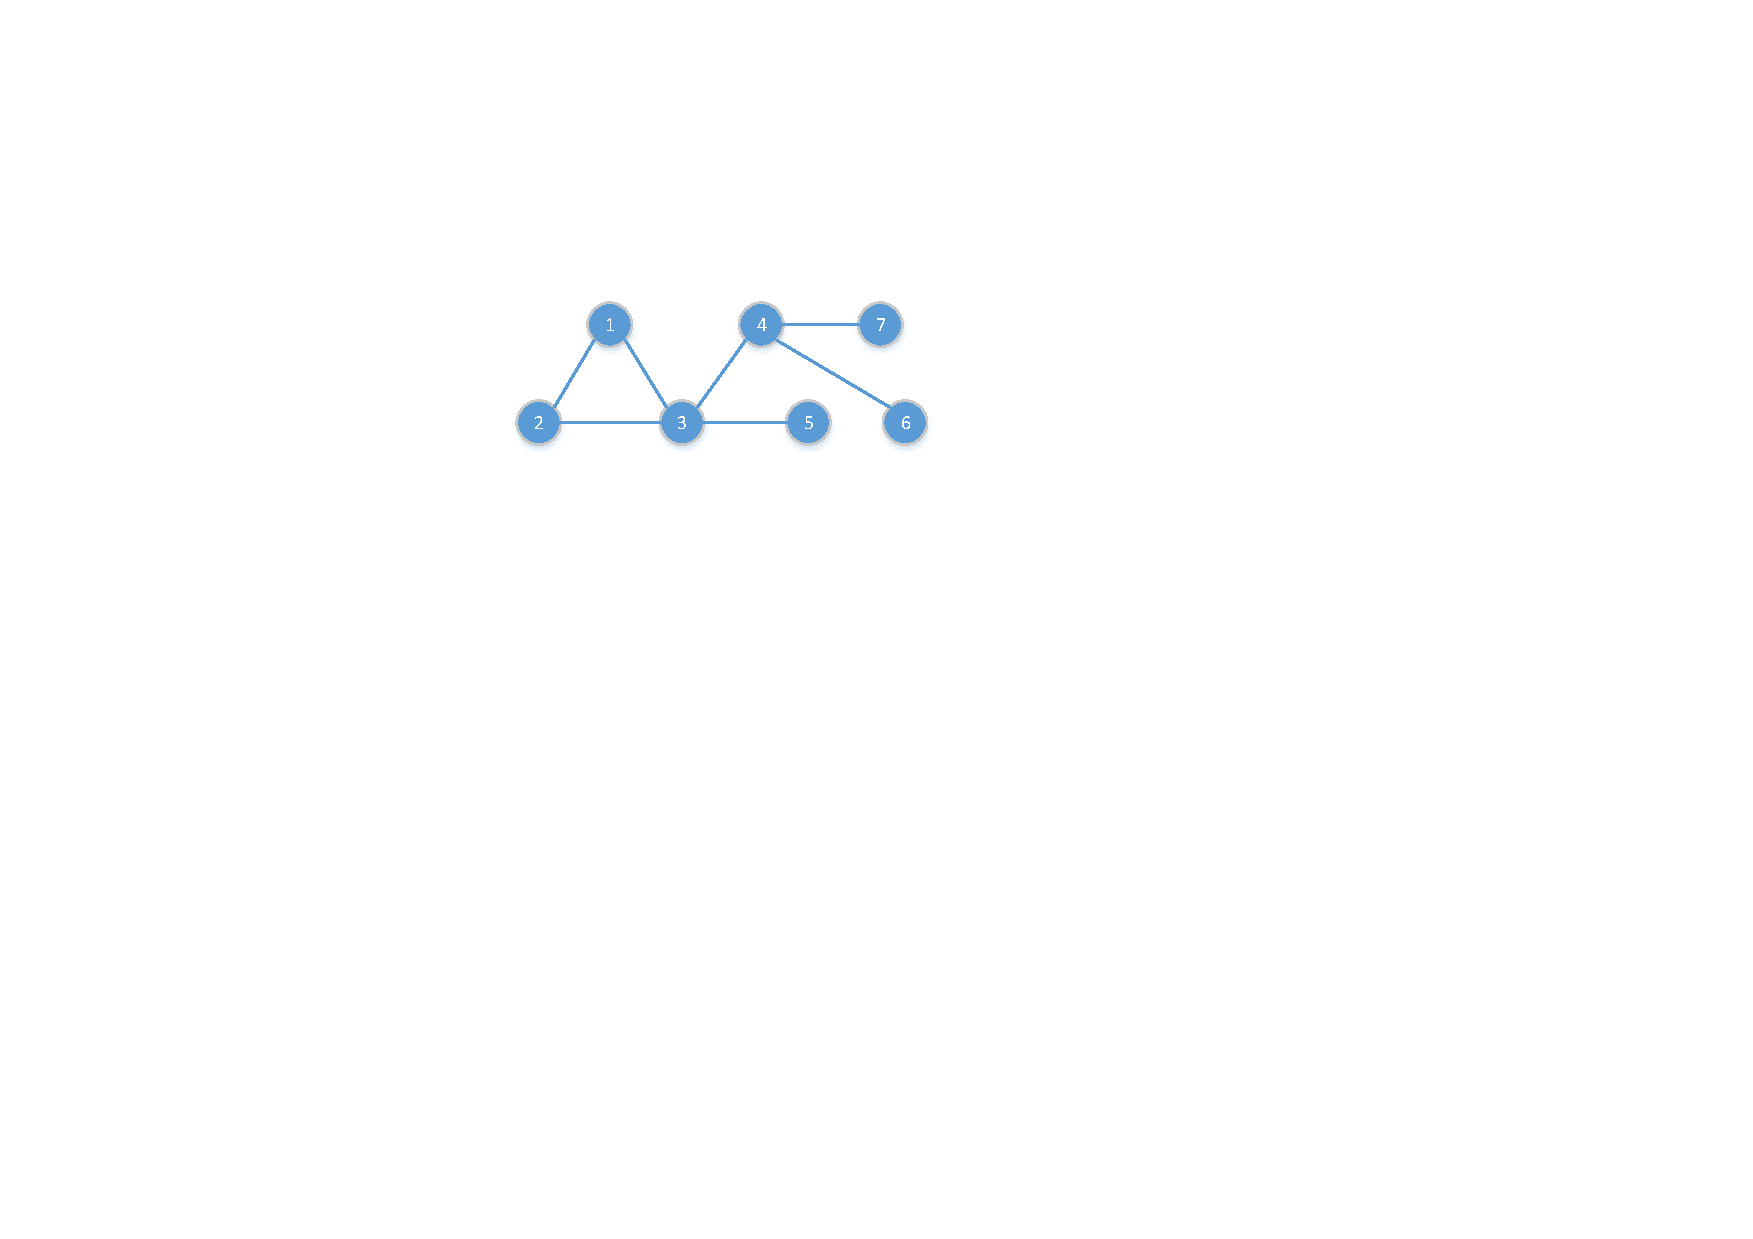
\includegraphics[scale=0.75]{./figures/part1/undirected_graph.pdf}
       \label{fig:graph:ExampleGraphUndirected}%
       }
       \hspace{0.1in}
   \subfigure[][{有向图}]{%
      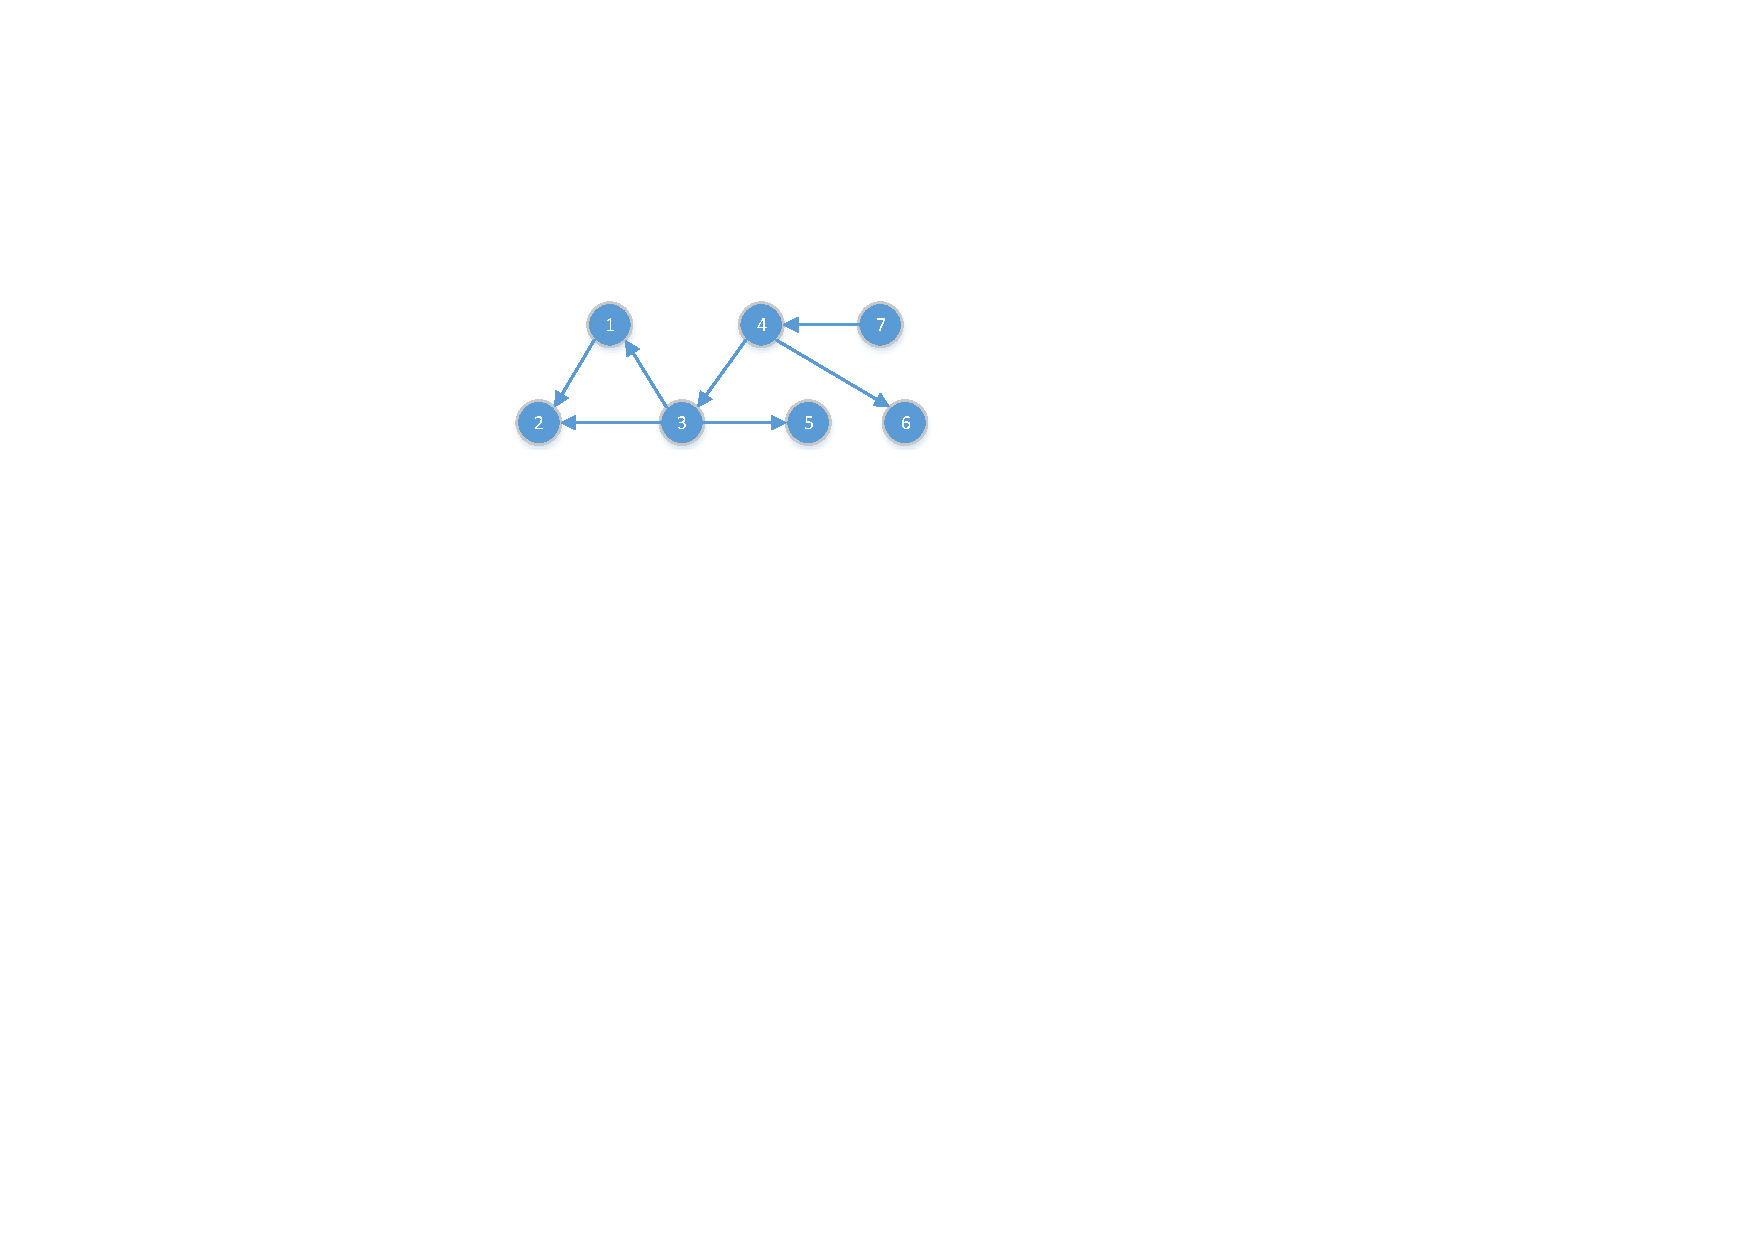
\includegraphics[scale=0.75]{./figures/part1/directed_graph.pdf}
       \label{fig:graph:ExampleGraphDirected}%
       }%
 \caption{ 图示例}%
\vspace{-0.2in}
 \label{fig:graph:ExampleGraph}
\end{figure}
\end{example}

图的表示方式有很多种。不同的表示方式适用于不同的应用。其中最常见的两种表示方式就是:\emph{邻接表}和\emph{邻接矩阵}。

给定图$G=(V,E)$,它的邻接表就是给出图中每个点相邻的相邻的点。
给定无权图$G=(V,E)$,其中$|V|=n$,且V中的点编号为$v_{1},v_2,...,v_{n}$,G的邻接矩阵$\mathbb{A}=[a_{i,j}]$是一个$n\times n$的0-1矩阵,它满足这样的性质:若存在一条边$e=(v_i,v_j)\in E$,则$a_{i,j}=1$;否则,$a_{i,j}=0$。若是有权图,若存在一条边$e=(v_i,v_j)\in E$,则$a_{i,j}=w(e)$。图\ref{fig:graph:ExampleGraphRepresentation}给出了图\ref{fig:graph:ExampleGraphUndirected}所示图的邻接表和邻接矩阵。

\begin{figure}[h]
   \centering
\subfigure[][{邻接表}]{%
      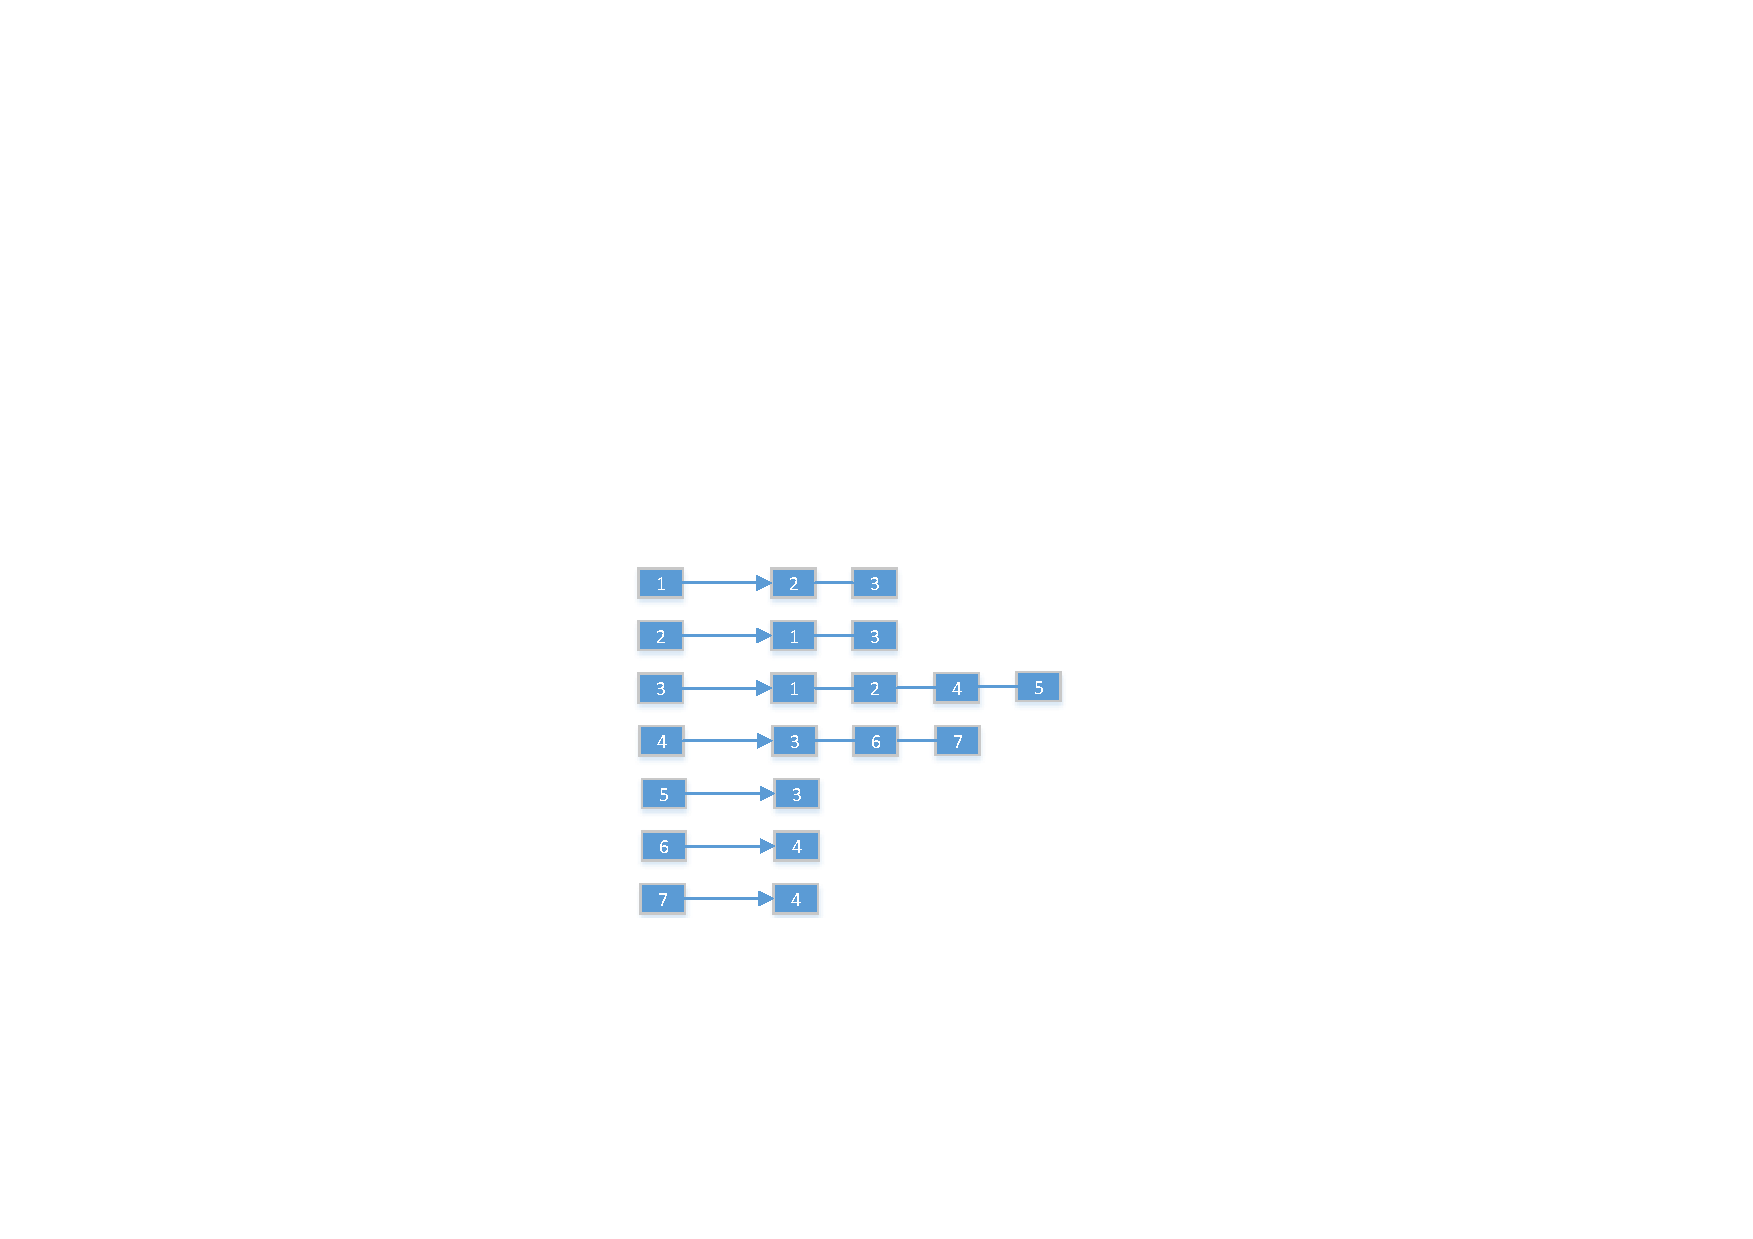
\includegraphics[scale=0.8]{./figures/part1/adjacent_list.pdf}
       \label{fig:graph:ExampleAdjacentList}%
       }
       \hspace{0.05in}
   \subfigure[][{邻接矩阵}]{%
      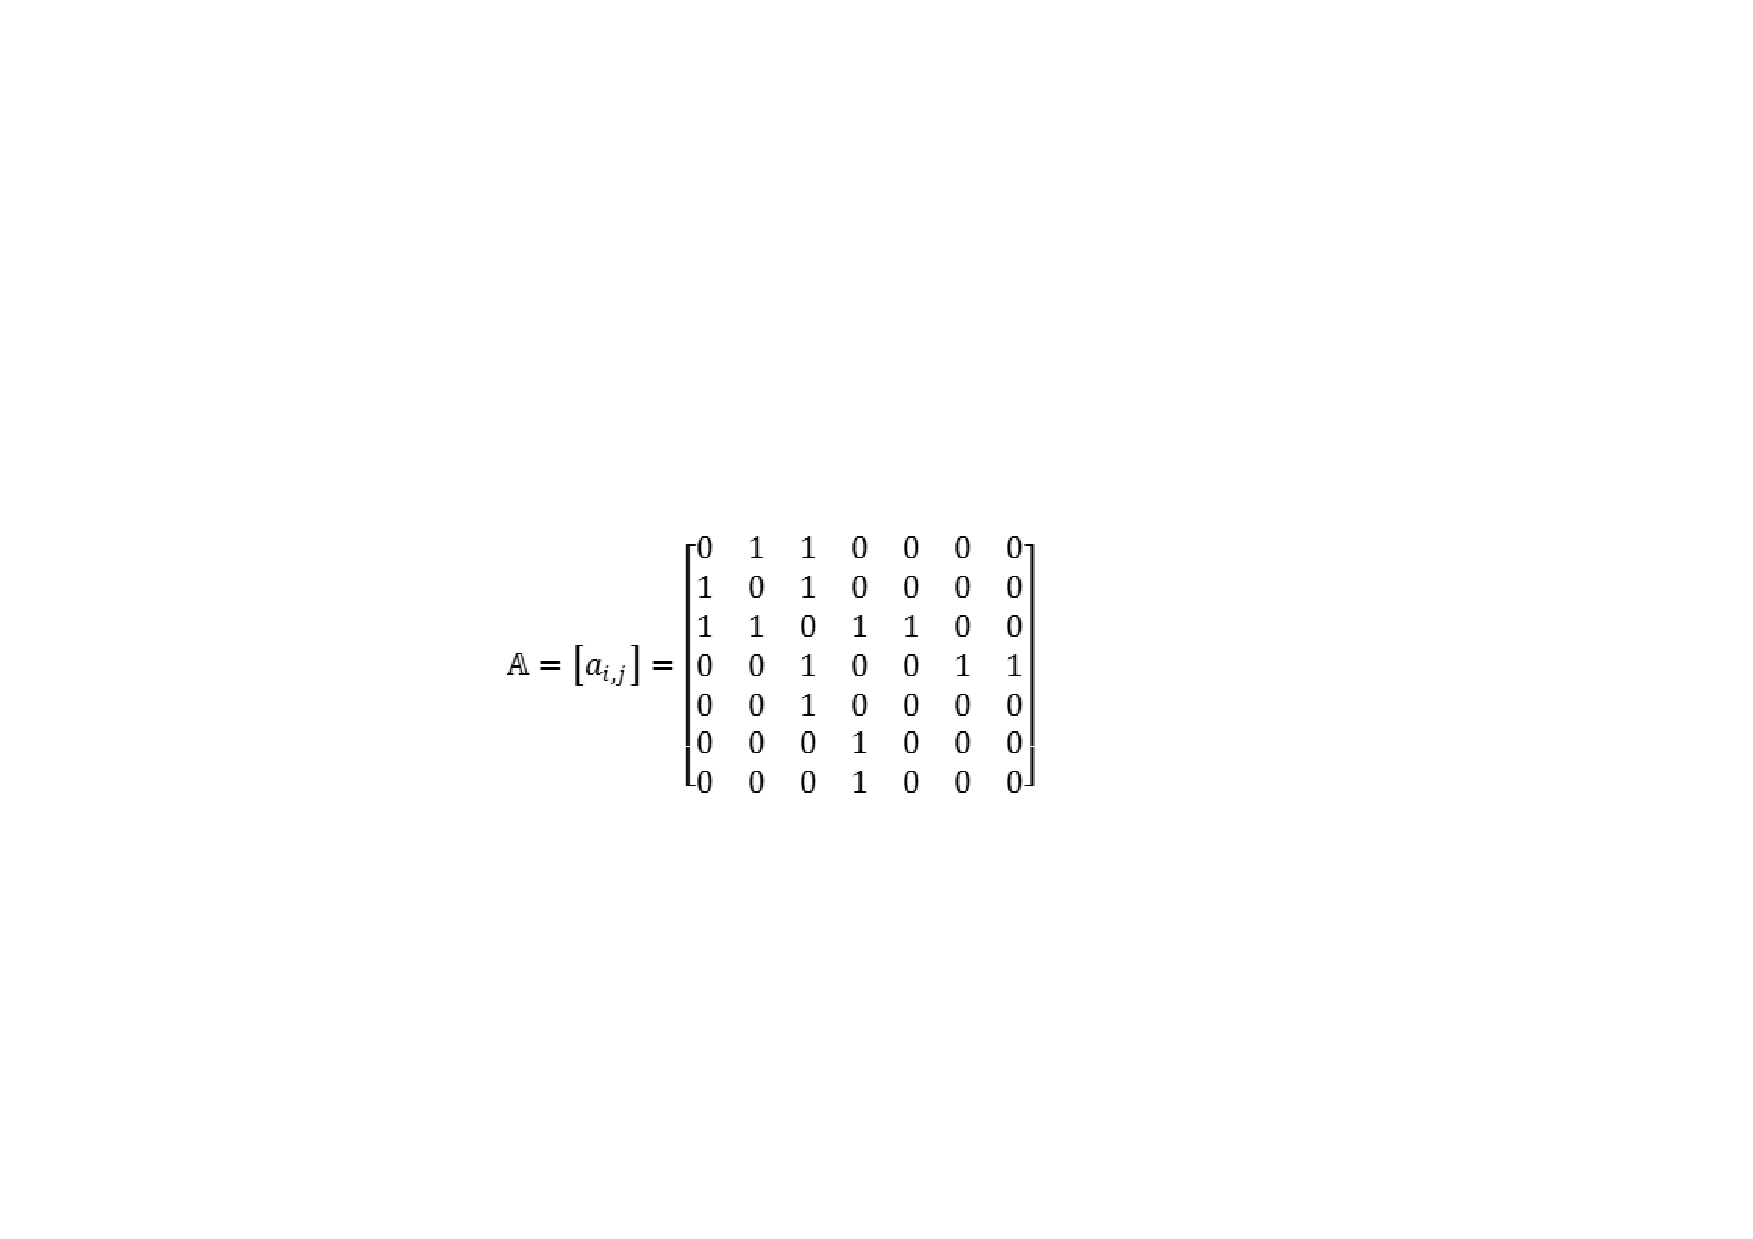
\includegraphics[scale=0.65]{./figures/part1/adjacent_matrix.pdf}
       \label{fig:graph:ExampleAdjacentMatrix}%
       }%
 \caption{ 图的表示方式示例}%
\vspace{-0.2in}
 \label{fig:graph:ExampleGraphRepresentation}
\end{figure}


此外,许多问题是利用沿图中的边前进所形成的的路径来建模的。例如,判定能否从一个公路网络中的某个点行进到另一个点,就可以用图中的路径概念来建模。
定义\ref{def:graph_path}给出了路径的形式化定义和相关术语。
\begin{definition}
\label{def:graph_path}
\textbf{路径}:给定一个无向图$G=(V,E)$,G中顶点与边的交替序列$\Gamma = v_{i_0}e_{j_1}v_{i_1}e_{j_2}...e_{j_l}v_{i_l}$称为点$v_{i_0}$到点$v_{i_l}$的\emph{路径},其中$v_{i_{r-1}}$和$v_{i_{r}}$是$e_{i_r}$的端点($1\le r\le l$)。点$v_{i_0}$和点$v_{i_l}$分别被称为$\Gamma$的起点和终点。若$v_{i_0}$和点$v_{i_l}$是同一个点,则$\Gamma$被称为一条\emph{回路}。
如果$G$中任意两个顶点之间都存在一条路径,则称该图为连通图,否则,称该图为非连通图。非连通图的极大连通子图称为它的连通分量。

若图G是无权图,$\Gamma$中的边数$l$被称为$\Gamma$ 的\emph{长度};若G是有权图,那么$\Gamma$中各条边权重之和$\sum_{k=1}^{k=l} w(e_{j_k})$就是$\Gamma$的\emph{长度}。所有$v_{i_0}$和点$v_{i_l}$之间的路径中最短的那条路径称为\emph{最短路径},最短路径的长度被称为$v_{i_0}$到点$v_{i_l}$的\emph{距离},记为$d(v_{i_0},v_{i_l})$。

有向图中的路径、长度和回路的定义与无向图中定义类似,只是要注意在有向图中路径和回路中边的方向的一致性,即在$\Gamma = v_{i_0}e_{j_1}v_{i_1}e_{j_2}...e_{j_l}v_{i_l}$中,$v_{i_{r-1}}$必须是$e_{i_r}$的起点且$v_{i_{r}}$是$e_{i_r}$的终点($1\le r\le l$)。此外,若对于有向图G中任意两个不同的顶点$v_i$和$v_j$,都存在从$v_i$到$v_j$以及从$v_j$到$v_i$的路径,则称G是强连通图。有向图的极大强连通子图称为它的强连通分量。
\end{definition}

\subsection{图遍历问题}
图遍历又称图的遍历,指的是从图中的任一顶点出发,对图中的所有顶点访问一次且只访问一次。图的遍历是图的一种基本操作,图的许多其它操作都是建立在遍历操作的基础之上。



由于图本身的复杂性,所以图的遍历操作也较复杂,主要表现在以下几个方面:


\begin{itemize}
  \item 在图中,没有一个“自然”的首结点,图中任意一个顶点都可作为第一个被访问的结点;
  \item 在有向图中,从一个顶点出发,只能够访问它所在的连通分量上的所有顶点,所以为了访问所有点还需考虑如何选取下一个出发点。在无向图中,从一个顶点出发,能够访问它所在的连通分量上的所有顶点,所以为了访问所有点还需考虑如何选取其他连通分量的下一个出发点。
  \item 在图结构中,如果有回路存在,那么一个顶点被访问之后,有可能沿回路又回到该顶点;
\end{itemize}

在图中,一个顶点可以和其它多个顶点相连,当这样的顶点访问过后,存在如何选取下一个要访问的顶点的问题。根据不同选取策略,图遍历算法可以分为:深度优先遍历和广度优先遍历。

\subsubsection{宽度优先遍历}

宽度优先搜索算法(又称广度优先搜索)是最简便的图的搜索算法之一,属于一种盲目搜寻法,目的是系统地展开并检查图中的所有节点,以找寻结果。换句话说,它并不考虑结果的可能位置,彻底地搜索整张图,直到找到结果为止。


\begin{algorithm}[h] \label{alg:BFS}
\caption{宽度优先遍历}
\small
\KwIn{图$G=(V,E,L)$和遍历起点$s$}
%\KwOut{ A set ${L_{in}}\subseteq L$ for coarsening}
$level[s] \gets 0$;\\
$parent[s] \gets s$;\\
将$s$插入队列queue中;\\
\While{$queue$不为空}{
	将队列queue的首个元素$v$推出;\\
	\For{$v$的相邻点$v^\prime$}{
		\If{$v$不在level中}{
			$level[v^\prime] \gets level[v^\prime] + 1$;\\
			$parent[v^\prime] \gets v$;\\
			将$v^\prime$插入队列queue中;\\
		}
	}
}
\end{algorithm}


\subsubsection{深度优先遍历}
深度优先遍历方法在于对每一个可能的分支路径深入到不能再深入为止,而且每个节点只能访问一次。它的基本思想是:从图的某个顶点$v_0$出发,访问$v_0$,然后选择一个与$v_0$相邻且没被访问过的顶点$v_i$访问,再从$v_i$出发选择一个与$v_i$相邻且未被访问的顶点$v_j$进行访问,依次继续。如果当前被访问过的顶点的所有邻接顶点都已被访问,则退回到已被访问的顶点序列中最后一个拥有未被访问的相邻顶点的顶点$w$,从$w$出发按同样的方法向前遍历,直到图中所有顶点都被访问。


\begin{algorithm}[h] \label{alg:DFS}
\caption{深度优先遍历和遍历起点$s$}
\small
\KwIn{图$G=(V,E,L)$和遍历起点$s$}
%\KwOut{ A set ${L_{in}}\subseteq L$ for coarsening}
$level[s] \gets 0$;\\
$parent[s] \gets s$;\\
将$s$插入栈stack中;\\
\While{$stack$不为空}{
	将栈stack的栈顶元素$v$推出;\\
	\For{$v$的相邻点$v^\prime$}{
		\If{$v$不在level中}{
			$level[v^\prime] \gets level[v^\prime] + 1$;\\
			$parent[v^\prime] \gets v$;\\
			将$v^\prime$插入栈stack中;\\
		}
	}
}
\end{algorithm}



\subsection{子图匹配问题}

\section{数据库}
数据库实际上就是一个文件集合,是一个存储数据的仓库,本质就是一个文件系统,数据库是按照特定的格式把数据存储起来,用户可以对存储的数据进行增删改查操作。

数据是指描述事物的符号记录,包括数据的表现形式和数据解释两个部分。如数字、音频、图形、文本、图像、语言、视频等多种表现形式。经过数字化处理后存入计算机。

数据是信息的符号表示或载体。信息是数据的内涵是对数据的语义解释。

数据库(DB):长期存储在计算机内、有组织、可共享的大量数据的集合。数据库中的数据按照一定的数据模型组织、描述和存储,具有娇小的冗余度、交稿的数据独立性和易扩展性,并可为各种用户共享。

数据库管理系统(DBMS):位于用户和操作系统间的数据管理系统的一层数据管理软件。用途:科学地组织和存储数据,高效地获取和维护数据。包括数据定义功能,数据组织、存储和管理,数据库的事物管理和运行管理,数据库的建立和维护功能,其他功能。

数据库系统(DBS):在计算机系统中引入数据库后的系统,一般由数据库。数据库管理系统(及其开发工具)、应用系统、数据库管理员构成。目的:存储信息并支持用户检索和更新所需的信息。

关系数据结构:描述现实世界的实体以及实体间的各种联系。只包含单一的数据结构—关系。

关系操作
查询操作:选择、投影、连接、除、并、差、交、笛卡尔积等。
插入、删除、修改操作。

关系的完整性约束
实体完整性和参照完整性:关系模型必须满足的完整性约束条件称为关系的两个不变性,应该由关系系统自动支持。
用户定义的完整性:应用领域需要遵循的约束条件,体现了具体领域中的语义约束。


SQL

